\documentclass[1p]{elsarticle_modified}
%\bibliographystyle{elsarticle-num}

%\usepackage[colorlinks]{hyperref}
%\usepackage{abbrmath_seonhwa} %\Abb, \Ascr, \Acal ,\Abf, \Afrak
\usepackage{amsfonts}
\usepackage{amssymb}
\usepackage{amsmath}
\usepackage{amsthm}
\usepackage{scalefnt}
\usepackage{amsbsy}
\usepackage{kotex}
\usepackage{caption}
\usepackage{subfig}
\usepackage{color}
\usepackage{graphicx}
\usepackage{xcolor} %% white, black, red, green, blue, cyan, magenta, yellow
\usepackage{float}
\usepackage{setspace}
\usepackage{hyperref}

\usepackage{tikz}
\usetikzlibrary{arrows}

\usepackage{multirow}
\usepackage{array} % fixed length table
\usepackage{hhline}

%%%%%%%%%%%%%%%%%%%%%
\makeatletter
\renewcommand*\env@matrix[1][\arraystretch]{%
	\edef\arraystretch{#1}%
	\hskip -\arraycolsep
	\let\@ifnextchar\new@ifnextchar
	\array{*\c@MaxMatrixCols c}}
\makeatother %https://tex.stackexchange.com/questions/14071/how-can-i-increase-the-line-spacing-in-a-matrix
%%%%%%%%%%%%%%%

\usepackage[normalem]{ulem}

\newcommand{\msout}[1]{\ifmmode\text{\sout{\ensuremath{#1}}}\else\sout{#1}\fi}
%SOURCE: \msout is \stkout macro in https://tex.stackexchange.com/questions/20609/strikeout-in-math-mode

\newcommand{\cancel}[1]{
	\ifmmode
	{\color{red}\msout{#1}}
	\else
	{\color{red}\sout{#1}}
	\fi
}

\newcommand{\add}[1]{
	{\color{blue}\uwave{#1}}
}

\newcommand{\replace}[2]{
	\ifmmode
	{\color{red}\msout{#1}}{\color{blue}\uwave{#2}}
	\else
	{\color{red}\sout{#1}}{\color{blue}\uwave{#2}}
	\fi
}

\newcommand{\Sol}{\mathcal{S}} %segment
\newcommand{\D}{D} %diagram
\newcommand{\A}{\mathcal{A}} %arc


%%%%%%%%%%%%%%%%%%%%%%%%%%%%%5 test

\def\sl{\operatorname{\textup{SL}}(2,\Cbb)}
\def\psl{\operatorname{\textup{PSL}}(2,\Cbb)}
\def\quan{\mkern 1mu \triangleright \mkern 1mu}

\theoremstyle{definition}
\newtheorem{thm}{Theorem}[section]
\newtheorem{prop}[thm]{Proposition}
\newtheorem{lem}[thm]{Lemma}
\newtheorem{ques}[thm]{Question}
\newtheorem{cor}[thm]{Corollary}
\newtheorem{defn}[thm]{Definition}
\newtheorem{exam}[thm]{Example}
\newtheorem{rmk}[thm]{Remark}
\newtheorem{alg}[thm]{Algorithm}

\newcommand{\I}{\sqrt{-1}}
\begin{document}

%\begin{frontmatter}
%
%\title{Boundary parabolic representations of knots up to 8 crossings}
%
%%% Group authors per affiliation:
%\author{Yunhi Cho} 
%\address{Department of Mathematics, University of Seoul, Seoul, Korea}
%\ead{yhcho@uos.ac.kr}
%
%
%\author{Seonhwa Kim} %\fnref{s_kim}}
%\address{Center for Geometry and Physics, Institute for Basic Science, Pohang, 37673, Korea}
%\ead{ryeona17@ibs.re.kr}
%
%\author{Hyuk Kim}
%\address{Department of Mathematical Sciences, Seoul National University, Seoul 08826, Korea}
%\ead{hyukkim@snu.ac.kr}
%
%\author{Seokbeom Yoon}
%\address{Department of Mathematical Sciences, Seoul National University, Seoul, 08826,  Korea}
%\ead{sbyoon15@snu.ac.kr}
%
%\begin{abstract}
%We find all boundary parabolic representation of knots up to 8 crossings.
%
%\end{abstract}
%\begin{keyword}
%    \MSC[2010] 57M25 
%\end{keyword}
%
%\end{frontmatter}

%\linenumbers
%\tableofcontents
%
\newcommand\colored[1]{\textcolor{white}{\rule[-0.35ex]{0.8em}{1.4ex}}\kern-0.8em\color{red} #1}%
%\newcommand\colored[1]{\textcolor{white}{ #1}\kern-2.17ex	\textcolor{white}{ #1}\kern-1.81ex	\textcolor{white}{ #1}\kern-2.15ex\color{red}#1	}

{\Large $\underline{12n_{0687}~(K12n_{0687})}$}

\setlength{\tabcolsep}{10pt}
\renewcommand{\arraystretch}{1.6}
\vspace{1cm}\begin{tabular}{m{100pt}>{\centering\arraybackslash}m{274pt}}
\multirow{5}{120pt}{
	\centering
	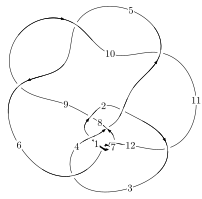
\includegraphics[width=112pt]{../../../GIT/diagram.site/Diagrams/png/2776_12n_0687.png}\\
\ \ \ A knot diagram\footnotemark}&
\allowdisplaybreaks
\textbf{Linearized knot diagam} \\
\cline{2-2}
 &
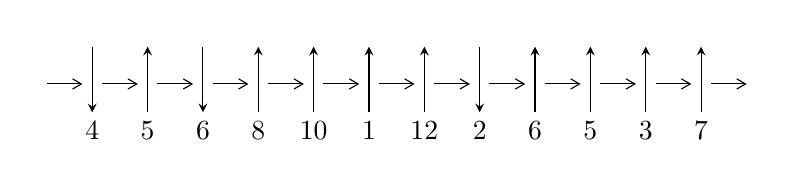
\begin{tikzpicture}[x=20pt, y=17pt]
	% nodes
	\node (C0) at (0, 0) {};
	\node (C1) at (1, 0) {};
	\node (C1U) at (1, +1) {};
	\node (C1D) at (1, -1) {4};

	\node (C2) at (2, 0) {};
	\node (C2U) at (2, +1) {};
	\node (C2D) at (2, -1) {5};

	\node (C3) at (3, 0) {};
	\node (C3U) at (3, +1) {};
	\node (C3D) at (3, -1) {6};

	\node (C4) at (4, 0) {};
	\node (C4U) at (4, +1) {};
	\node (C4D) at (4, -1) {8};

	\node (C5) at (5, 0) {};
	\node (C5U) at (5, +1) {};
	\node (C5D) at (5, -1) {10};

	\node (C6) at (6, 0) {};
	\node (C6U) at (6, +1) {};
	\node (C6D) at (6, -1) {1};

	\node (C7) at (7, 0) {};
	\node (C7U) at (7, +1) {};
	\node (C7D) at (7, -1) {12};

	\node (C8) at (8, 0) {};
	\node (C8U) at (8, +1) {};
	\node (C8D) at (8, -1) {2};

	\node (C9) at (9, 0) {};
	\node (C9U) at (9, +1) {};
	\node (C9D) at (9, -1) {6};

	\node (C10) at (10, 0) {};
	\node (C10U) at (10, +1) {};
	\node (C10D) at (10, -1) {5};

	\node (C11) at (11, 0) {};
	\node (C11U) at (11, +1) {};
	\node (C11D) at (11, -1) {3};

	\node (C12) at (12, 0) {};
	\node (C12U) at (12, +1) {};
	\node (C12D) at (12, -1) {7};
	\node (C13) at (13, 0) {};

	% arrows
	\draw[->,>={angle 60}]
	(C0) edge (C1) (C1) edge (C2) (C2) edge (C3) (C3) edge (C4) (C4) edge (C5) (C5) edge (C6) (C6) edge (C7) (C7) edge (C8) (C8) edge (C9) (C9) edge (C10) (C10) edge (C11) (C11) edge (C12) (C12) edge (C13) ;	\draw[->,>=stealth]
	(C1U) edge (C1D) (C2D) edge (C2U) (C3U) edge (C3D) (C4D) edge (C4U) (C5D) edge (C5U) (C6D) edge (C6U) (C7D) edge (C7U) (C8U) edge (C8D) (C9D) edge (C9U) (C10D) edge (C10U) (C11D) edge (C11U) (C12D) edge (C12U) ;
	\end{tikzpicture} \\
\hhline{~~} \\& 
\textbf{Solving Sequence} \\ \cline{2-2} 
 &
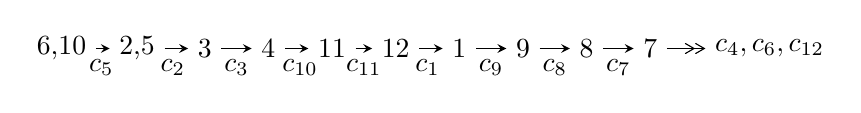
\begin{tikzpicture}[x=23pt, y=7pt]
	% node
	\node (A0) at (-1/8, 0) {6,10};
	\node (A1) at (17/16, 0) {2,5};
	\node (A2) at (17/8, 0) {3};
	\node (A3) at (25/8, 0) {4};
	\node (A4) at (33/8, 0) {11};
	\node (A5) at (41/8, 0) {12};
	\node (A6) at (49/8, 0) {1};
	\node (A7) at (57/8, 0) {9};
	\node (A8) at (65/8, 0) {8};
	\node (A9) at (73/8, 0) {7};
	\node (C1) at (1/2, -1) {$c_{5}$};
	\node (C2) at (13/8, -1) {$c_{2}$};
	\node (C3) at (21/8, -1) {$c_{3}$};
	\node (C4) at (29/8, -1) {$c_{10}$};
	\node (C5) at (37/8, -1) {$c_{11}$};
	\node (C6) at (45/8, -1) {$c_{1}$};
	\node (C7) at (53/8, -1) {$c_{9}$};
	\node (C8) at (61/8, -1) {$c_{8}$};
	\node (C9) at (69/8, -1) {$c_{7}$};
	\node (A10) at (11, 0) {$c_{4},c_{6},c_{12}$};

	% edge
	\draw[->,>=stealth]	
	(A0) edge (A1) (A1) edge (A2) (A2) edge (A3) (A3) edge (A4) (A4) edge (A5) (A5) edge (A6) (A6) edge (A7) (A7) edge (A8) (A8) edge (A9) ;
	\draw[->>,>={angle 60}]	
	(A9) edge (A10);
\end{tikzpicture} \\ 

\end{tabular} \\

\footnotetext{
The image of knot diagram is generated by the software ``\textbf{Draw programme}" developed by Andrew Bartholomew(\url{http://www.layer8.co.uk/maths/draw/index.htm\#Running-draw}), where we modified some parts for our purpose(\url{https://github.com/CATsTAILs/LinksPainter}).
}\phantom \\ \newline 
\centering \textbf{Ideals for irreducible components\footnotemark of $X_{\text{par}}$} 
 
\begin{align*}
I^u_{1}&=\langle 
9.93374\times10^{151} u^{69}-5.73011\times10^{151} u^{68}+\cdots+1.25167\times10^{152} b-1.15684\times10^{152},\\
\phantom{I^u_{1}}&\phantom{= \langle  }-2.27978\times10^{152} u^{69}+7.27815\times10^{151} u^{68}+\cdots+1.25167\times10^{152} a-1.09032\times10^{153},\\
\phantom{I^u_{1}}&\phantom{= \langle  }u^{70}+8 u^{68}+\cdots+12 u+1\rangle \\
I^u_{2}&=\langle 
784 u^{16}-1472 u^{15}+\cdots+281 b-1616,\;- u^{16}-4 u^{14}+\cdots+a-7,\;u^{17}- u^{16}+\cdots- u+1\rangle \\
\\
\end{align*}
\raggedright * 2 irreducible components of $\dim_{\mathbb{C}}=0$, with total 87 representations.\\
\footnotetext{All coefficients of polynomials are rational numbers. But the coefficients are sometimes approximated in decimal forms when there is not enough margin.}
\newpage
\renewcommand{\arraystretch}{1}
\centering \section*{I. $I^u_{1}= \langle 9.93\times10^{151} u^{69}-5.73\times10^{151} u^{68}+\cdots+1.25\times10^{152} b-1.16\times10^{152},\;-2.28\times10^{152} u^{69}+7.28\times10^{151} u^{68}+\cdots+1.25\times10^{152} a-1.09\times10^{153},\;u^{70}+8 u^{68}+\cdots+12 u+1 \rangle$}
\flushleft \textbf{(i) Arc colorings}\\
\begin{tabular}{m{7pt} m{180pt} m{7pt} m{180pt} }
\flushright $a_{6}=$&$\begin{pmatrix}1\\0\end{pmatrix}$ \\
\flushright $a_{10}=$&$\begin{pmatrix}0\\u\end{pmatrix}$ \\
\flushright $a_{2}=$&$\begin{pmatrix}1.82140 u^{69}-0.581477 u^{68}+\cdots+39.0109 u+8.71095\\-0.793642 u^{69}+0.457798 u^{68}+\cdots+1.47985 u+0.924244\end{pmatrix}$ \\
\flushright $a_{5}=$&$\begin{pmatrix}1\\u^2\end{pmatrix}$ \\
\flushright $a_{3}=$&$\begin{pmatrix}1.02178 u^{69}-0.283802 u^{68}+\cdots+35.3344 u+9.05372\\-0.484690 u^{69}+0.265454 u^{68}+\cdots-1.29264 u+0.626569\end{pmatrix}$ \\
\flushright $a_{4}=$&$\begin{pmatrix}1.50647 u^{69}-0.549256 u^{68}+\cdots+36.6270 u+8.42715\\-0.484690 u^{69}+0.265454 u^{68}+\cdots-1.29264 u+0.626569\end{pmatrix}$ \\
\flushright $a_{11}=$&$\begin{pmatrix}u\\u^3+u\end{pmatrix}$ \\
\flushright $a_{12}=$&$\begin{pmatrix}-2.10413 u^{69}+0.456635 u^{68}+\cdots-57.5910 u-11.5890\\0.171585 u^{69}+0.157443 u^{68}+\cdots-6.10514 u-1.41447\end{pmatrix}$ \\
\flushright $a_{1}=$&$\begin{pmatrix}1.13758 u^{69}-0.539841 u^{68}+\cdots+39.0714 u+7.72721\\0.261369 u^{69}-0.0100471 u^{68}+\cdots-1.35091 u+0.206159\end{pmatrix}$ \\
\flushright $a_{9}=$&$\begin{pmatrix}- u\\u\end{pmatrix}$ \\
\flushright $a_{8}=$&$\begin{pmatrix}-1.63790 u^{69}+0.361732 u^{68}+\cdots-57.8284 u-11.6027\\-0.708579 u^{69}-0.0963778 u^{68}+\cdots-16.6684 u-2.12525\end{pmatrix}$ \\
\flushright $a_{7}=$&$\begin{pmatrix}-1.39909 u^{69}+0.856722 u^{68}+\cdots-38.1398 u-5.68756\\-0.279079 u^{69}-0.230487 u^{68}+\cdots-17.0325 u-1.58453\end{pmatrix}$\\&\end{tabular}
\flushleft \textbf{(ii) Obstruction class $= -1$}\\~\\
\flushleft \textbf{(iii) Cusp Shapes $= -0.717657 u^{69}+2.08595 u^{68}+\cdots+98.0282 u+17.8328$}\\~\\
\newpage\renewcommand{\arraystretch}{1}
\flushleft \textbf{(iv) u-Polynomials at the component}\newline \\
\begin{tabular}{m{50pt}|m{274pt}}
Crossings & \hspace{64pt}u-Polynomials at each crossing \\
\hline $$\begin{aligned}c_{1}\end{aligned}$$&$\begin{aligned}
&u^{70}-8 u^{69}+\cdots+54 u+9
\end{aligned}$\\
\hline $$\begin{aligned}c_{2}\end{aligned}$$&$\begin{aligned}
&u^{70}-7 u^{69}+\cdots+9260 u-7239
\end{aligned}$\\
\hline $$\begin{aligned}c_{3}\end{aligned}$$&$\begin{aligned}
&u^{70}+2 u^{69}+\cdots+564 u+41
\end{aligned}$\\
\hline $$\begin{aligned}c_{4}\end{aligned}$$&$\begin{aligned}
&u^{70}- u^{69}+\cdots-22 u-1
\end{aligned}$\\
\hline $$\begin{aligned}c_{5},c_{9},c_{10}\end{aligned}$$&$\begin{aligned}
&u^{70}+8 u^{68}+\cdots-12 u+1
\end{aligned}$\\
\hline $$\begin{aligned}c_{6},c_{7},c_{12}\end{aligned}$$&$\begin{aligned}
&u^{70}+34 u^{68}+\cdots+17 u+3
\end{aligned}$\\
\hline $$\begin{aligned}c_{8}\end{aligned}$$&$\begin{aligned}
&u^{70}-2 u^{69}+\cdots+4105 u+2083
\end{aligned}$\\
\hline $$\begin{aligned}c_{11}\end{aligned}$$&$\begin{aligned}
&u^{70}+u^{69}+\cdots-329 u+1651
\end{aligned}$\\
\hline
\end{tabular}\\~\\
\newpage\renewcommand{\arraystretch}{1}
\flushleft \textbf{(v) Riley Polynomials at the component}\newline \\
\begin{tabular}{m{50pt}|m{274pt}}
Crossings & \hspace{64pt}Riley Polynomials at each crossing \\
\hline $$\begin{aligned}c_{1}\end{aligned}$$&$\begin{aligned}
&y^{70}-10 y^{69}+\cdots-144 y+81
\end{aligned}$\\
\hline $$\begin{aligned}c_{2}\end{aligned}$$&$\begin{aligned}
&y^{70}-61 y^{69}+\cdots-1022459722 y+52403121
\end{aligned}$\\
\hline $$\begin{aligned}c_{3}\end{aligned}$$&$\begin{aligned}
&y^{70}+12 y^{69}+\cdots-24782 y+1681
\end{aligned}$\\
\hline $$\begin{aligned}c_{4}\end{aligned}$$&$\begin{aligned}
&y^{70}+7 y^{69}+\cdots+122 y+1
\end{aligned}$\\
\hline $$\begin{aligned}c_{5},c_{9},c_{10}\end{aligned}$$&$\begin{aligned}
&y^{70}+16 y^{69}+\cdots-30 y+1
\end{aligned}$\\
\hline $$\begin{aligned}c_{6},c_{7},c_{12}\end{aligned}$$&$\begin{aligned}
&y^{70}+68 y^{69}+\cdots-223 y+9
\end{aligned}$\\
\hline $$\begin{aligned}c_{8}\end{aligned}$$&$\begin{aligned}
&y^{70}+12 y^{69}+\cdots+246685969 y+4338889
\end{aligned}$\\
\hline $$\begin{aligned}c_{11}\end{aligned}$$&$\begin{aligned}
&y^{70}-65 y^{69}+\cdots-76523125 y+2725801
\end{aligned}$\\
\hline
\end{tabular}\\~\\
\newpage\flushleft \textbf{(vi) Complex Volumes and Cusp Shapes}
$$\begin{array}{c|c|c}  
\text{Solutions to }I^u_{1}& \I (\text{vol} + \sqrt{-1}CS) & \text{Cusp shape}\\
 \hline 
\begin{aligned}
u &= \phantom{-}0.182629 + 0.959522 I \\
a &= \phantom{-}1.001330 + 0.504116 I \\
b &= -0.495567 + 0.539126 I\end{aligned}
 & -5.19104 + 2.89870 I & -1.83556 - 3.69030 I \\ \hline\begin{aligned}
u &= \phantom{-}0.182629 - 0.959522 I \\
a &= \phantom{-}1.001330 - 0.504116 I \\
b &= -0.495567 - 0.539126 I\end{aligned}
 & -5.19104 - 2.89870 I & -1.83556 + 3.69030 I \\ \hline\begin{aligned}
u &= \phantom{-}0.889971 + 0.615220 I \\
a &= \phantom{-}1.49599 - 0.81473 I \\
b &= \phantom{-}0.658738 + 0.726934 I\end{aligned}
 & -2.94953 + 6.14576 I & \phantom{-0.000000 } 0 \\ \hline\begin{aligned}
u &= \phantom{-}0.889971 - 0.615220 I \\
a &= \phantom{-}1.49599 + 0.81473 I \\
b &= \phantom{-}0.658738 - 0.726934 I\end{aligned}
 & -2.94953 - 6.14576 I & \phantom{-0.000000 } 0 \\ \hline\begin{aligned}
u &= \phantom{-}0.467157 + 1.015360 I \\
a &= \phantom{-}0.469020 - 0.334689 I \\
b &= -0.91014 + 1.45911 I\end{aligned}
 & -4.76852 - 0.93744 I & \phantom{-0.000000 } 0 \\ \hline\begin{aligned}
u &= \phantom{-}0.467157 - 1.015360 I \\
a &= \phantom{-}0.469020 + 0.334689 I \\
b &= -0.91014 - 1.45911 I\end{aligned}
 & -4.76852 + 0.93744 I & \phantom{-0.000000 } 0 \\ \hline\begin{aligned}
u &= -0.222651 + 0.847009 I \\
a &= \phantom{-}1.14984 + 1.14399 I \\
b &= -0.0748484 + 0.0360553 I\end{aligned}
 & -7.73355 + 3.72028 I & -2.51438 - 0.93811 I \\ \hline\begin{aligned}
u &= -0.222651 - 0.847009 I \\
a &= \phantom{-}1.14984 - 1.14399 I \\
b &= -0.0748484 - 0.0360553 I\end{aligned}
 & -7.73355 - 3.72028 I & -2.51438 + 0.93811 I \\ \hline\begin{aligned}
u &= -0.751668 + 0.837280 I \\
a &= -1.72961 - 0.46280 I \\
b &= \phantom{-}1.14330 + 1.25142 I\end{aligned}
 & -0.30303 - 6.28207 I & \phantom{-0.000000 } 0 \\ \hline\begin{aligned}
u &= -0.751668 - 0.837280 I \\
a &= -1.72961 + 0.46280 I \\
b &= \phantom{-}1.14330 - 1.25142 I\end{aligned}
 & -0.30303 + 6.28207 I & \phantom{-0.000000 } 0\\
 \hline 
 \end{array}$$\newpage$$\begin{array}{c|c|c}  
\text{Solutions to }I^u_{1}& \I (\text{vol} + \sqrt{-1}CS) & \text{Cusp shape}\\
 \hline 
\begin{aligned}
u &= \phantom{-}0.770010 + 0.372544 I \\
a &= \phantom{-}0.581630 - 0.055990 I \\
b &= \phantom{-}0.144106 + 0.825142 I\end{aligned}
 & -4.08900 + 2.25007 I & \phantom{-}3.53748 - 2.27099 I \\ \hline\begin{aligned}
u &= \phantom{-}0.770010 - 0.372544 I \\
a &= \phantom{-}0.581630 + 0.055990 I \\
b &= \phantom{-}0.144106 - 0.825142 I\end{aligned}
 & -4.08900 - 2.25007 I & \phantom{-}3.53748 + 2.27099 I \\ \hline\begin{aligned}
u &= -1.14498\phantom{ +0.000000I} \\
a &= \phantom{-}1.73239\phantom{ +0.000000I} \\
b &= \phantom{-}1.53512\phantom{ +0.000000I}\end{aligned}
 & \phantom{-}2.60015\phantom{ +0.000000I} & -58.8670\phantom{ +0.000000I} \\ \hline\begin{aligned}
u &= -0.268041 + 0.804909 I \\
a &= \phantom{-}0.542252 - 0.218224 I \\
b &= -0.423247 - 0.869174 I\end{aligned}
 & -0.98658 - 2.03464 I & \phantom{-}3.76283 + 3.73374 I \\ \hline\begin{aligned}
u &= -0.268041 - 0.804909 I \\
a &= \phantom{-}0.542252 + 0.218224 I \\
b &= -0.423247 + 0.869174 I\end{aligned}
 & -0.98658 + 2.03464 I & \phantom{-}3.76283 - 3.73374 I \\ \hline\begin{aligned}
u &= -0.656557 + 0.954242 I \\
a &= -0.493373 - 1.239310 I \\
b &= -0.00110 + 1.66937 I\end{aligned}
 & -0.681468 + 0.834270 I & \phantom{-0.000000 } 0 \\ \hline\begin{aligned}
u &= -0.656557 - 0.954242 I \\
a &= -0.493373 + 1.239310 I \\
b &= -0.00110 - 1.66937 I\end{aligned}
 & -0.681468 - 0.834270 I & \phantom{-0.000000 } 0 \\ \hline\begin{aligned}
u &= \phantom{-}0.825164 + 0.845513 I \\
a &= -1.40194 + 0.58938 I \\
b &= \phantom{-}0.92803 - 1.30897 I\end{aligned}
 & \phantom{-}4.72221 + 4.24472 I & \phantom{-0.000000 } 0 \\ \hline\begin{aligned}
u &= \phantom{-}0.825164 - 0.845513 I \\
a &= -1.40194 - 0.58938 I \\
b &= \phantom{-}0.92803 + 1.30897 I\end{aligned}
 & \phantom{-}4.72221 - 4.24472 I & \phantom{-0.000000 } 0 \\ \hline\begin{aligned}
u &= \phantom{-}1.068270 + 0.572212 I \\
a &= -0.776105 + 0.152158 I \\
b &= \phantom{-}0.735609 - 0.965380 I\end{aligned}
 & \phantom{-}0.233976 + 0.759074 I & \phantom{-0.000000 } 0\\
 \hline 
 \end{array}$$\newpage$$\begin{array}{c|c|c}  
\text{Solutions to }I^u_{1}& \I (\text{vol} + \sqrt{-1}CS) & \text{Cusp shape}\\
 \hline 
\begin{aligned}
u &= \phantom{-}1.068270 - 0.572212 I \\
a &= -0.776105 - 0.152158 I \\
b &= \phantom{-}0.735609 + 0.965380 I\end{aligned}
 & \phantom{-}0.233976 - 0.759074 I & \phantom{-0.000000 } 0 \\ \hline\begin{aligned}
u &= -0.819050 + 0.902886 I \\
a &= -1.25597 - 1.03649 I \\
b &= \phantom{-}0.75273 + 1.61897 I\end{aligned}
 & \phantom{-}1.70243 - 3.06412 I & \phantom{-0.000000 } 0 \\ \hline\begin{aligned}
u &= -0.819050 - 0.902886 I \\
a &= -1.25597 + 1.03649 I \\
b &= \phantom{-}0.75273 - 1.61897 I\end{aligned}
 & \phantom{-}1.70243 + 3.06412 I & \phantom{-0.000000 } 0 \\ \hline\begin{aligned}
u &= -0.532408 + 0.562547 I \\
a &= -0.491267 + 0.375201 I \\
b &= \phantom{-}0.05004 - 1.69837 I\end{aligned}
 & -6.45795 - 6.80158 I & \phantom{-}1.45639 + 9.56884 I \\ \hline\begin{aligned}
u &= -0.532408 - 0.562547 I \\
a &= -0.491267 - 0.375201 I \\
b &= \phantom{-}0.05004 + 1.69837 I\end{aligned}
 & -6.45795 + 6.80158 I & \phantom{-}1.45639 - 9.56884 I \\ \hline\begin{aligned}
u &= \phantom{-}0.763532 + 0.981407 I \\
a &= -0.747021 + 1.045390 I \\
b &= \phantom{-}0.29445 - 1.52258 I\end{aligned}
 & \phantom{-}4.29081 + 1.75973 I & \phantom{-0.000000 } 0 \\ \hline\begin{aligned}
u &= \phantom{-}0.763532 - 0.981407 I \\
a &= -0.747021 - 1.045390 I \\
b &= \phantom{-}0.29445 + 1.52258 I\end{aligned}
 & \phantom{-}4.29081 - 1.75973 I & \phantom{-0.000000 } 0 \\ \hline\begin{aligned}
u &= \phantom{-}0.031790 + 0.748955 I \\
a &= \phantom{-}1.337290 + 0.340343 I \\
b &= -1.69605 - 0.47490 I\end{aligned}
 & -2.07518 - 1.88050 I & -0.58788 + 2.54582 I \\ \hline\begin{aligned}
u &= \phantom{-}0.031790 - 0.748955 I \\
a &= \phantom{-}1.337290 - 0.340343 I \\
b &= -1.69605 + 0.47490 I\end{aligned}
 & -2.07518 + 1.88050 I & -0.58788 - 2.54582 I \\ \hline\begin{aligned}
u &= -1.026810 + 0.770847 I \\
a &= -0.931991 - 0.352914 I \\
b &= \phantom{-}0.727009 + 1.062520 I\end{aligned}
 & \phantom{-}4.78970 - 2.73592 I & \phantom{-0.000000 } 0\\
 \hline 
 \end{array}$$\newpage$$\begin{array}{c|c|c}  
\text{Solutions to }I^u_{1}& \I (\text{vol} + \sqrt{-1}CS) & \text{Cusp shape}\\
 \hline 
\begin{aligned}
u &= -1.026810 - 0.770847 I \\
a &= -0.931991 + 0.352914 I \\
b &= \phantom{-}0.727009 - 1.062520 I\end{aligned}
 & \phantom{-}4.78970 + 2.73592 I & \phantom{-0.000000 } 0 \\ \hline\begin{aligned}
u &= -0.076174 + 0.691781 I \\
a &= \phantom{-}1.76879 - 0.64957 I \\
b &= -2.25934 + 0.77220 I\end{aligned}
 & -8.05518 + 4.99038 I & -5.61415 + 0.00335 I \\ \hline\begin{aligned}
u &= -0.076174 - 0.691781 I \\
a &= \phantom{-}1.76879 + 0.64957 I \\
b &= -2.25934 - 0.77220 I\end{aligned}
 & -8.05518 - 4.99038 I & -5.61415 - 0.00335 I \\ \hline\begin{aligned}
u &= \phantom{-}0.403606 + 0.564847 I \\
a &= -0.472960 + 0.090622 I \\
b &= \phantom{-}0.124640 + 1.386760 I\end{aligned}
 & -0.86012 + 4.21216 I & \phantom{-}6.35099 - 11.74346 I \\ \hline\begin{aligned}
u &= \phantom{-}0.403606 - 0.564847 I \\
a &= -0.472960 - 0.090622 I \\
b &= \phantom{-}0.124640 - 1.386760 I\end{aligned}
 & -0.86012 - 4.21216 I & \phantom{-}6.35099 + 11.74346 I \\ \hline\begin{aligned}
u &= \phantom{-}0.019991 + 0.681568 I \\
a &= \phantom{-}0.664079 - 1.210490 I \\
b &= \phantom{-}0.074205 - 0.421986 I\end{aligned}
 & -1.57608 - 2.34912 I & \phantom{-}0.437437 + 0.644148 I \\ \hline\begin{aligned}
u &= \phantom{-}0.019991 - 0.681568 I \\
a &= \phantom{-}0.664079 + 1.210490 I \\
b &= \phantom{-}0.074205 + 0.421986 I\end{aligned}
 & -1.57608 + 2.34912 I & \phantom{-}0.437437 - 0.644148 I \\ \hline\begin{aligned}
u &= -0.316585 + 0.590067 I \\
a &= -3.02818 + 1.36465 I \\
b &= \phantom{-}1.287870 + 0.396140 I\end{aligned}
 & -7.54675 - 6.57227 I & -0.27416 + 11.76800 I \\ \hline\begin{aligned}
u &= -0.316585 - 0.590067 I \\
a &= -3.02818 - 1.36465 I \\
b &= \phantom{-}1.287870 - 0.396140 I\end{aligned}
 & -7.54675 + 6.57227 I & -0.27416 - 11.76800 I \\ \hline\begin{aligned}
u &= -1.075700 + 0.803829 I \\
a &= \phantom{-}1.005200 + 0.615424 I \\
b &= \phantom{-}0.311248 - 1.377500 I\end{aligned}
 & \phantom{-}4.84131 - 0.55610 I & \phantom{-0.000000 } 0\\
 \hline 
 \end{array}$$\newpage$$\begin{array}{c|c|c}  
\text{Solutions to }I^u_{1}& \I (\text{vol} + \sqrt{-1}CS) & \text{Cusp shape}\\
 \hline 
\begin{aligned}
u &= -1.075700 - 0.803829 I \\
a &= \phantom{-}1.005200 - 0.615424 I \\
b &= \phantom{-}0.311248 + 1.377500 I\end{aligned}
 & \phantom{-}4.84131 + 0.55610 I & \phantom{-0.000000 } 0 \\ \hline\begin{aligned}
u &= \phantom{-}0.902166 + 1.001410 I \\
a &= \phantom{-}1.057310 - 0.402054 I \\
b &= -0.42852 + 1.63869 I\end{aligned}
 & -4.61180 + 3.36092 I & \phantom{-0.000000 } 0 \\ \hline\begin{aligned}
u &= \phantom{-}0.902166 - 1.001410 I \\
a &= \phantom{-}1.057310 + 0.402054 I \\
b &= -0.42852 - 1.63869 I\end{aligned}
 & -4.61180 - 3.36092 I & \phantom{-0.000000 } 0 \\ \hline\begin{aligned}
u &= \phantom{-}1.093450 + 0.794950 I \\
a &= \phantom{-}0.905104 - 0.704207 I \\
b &= \phantom{-}0.255022 + 1.286370 I\end{aligned}
 & \phantom{-}5.66823 - 4.85184 I & \phantom{-0.000000 } 0 \\ \hline\begin{aligned}
u &= \phantom{-}1.093450 - 0.794950 I \\
a &= \phantom{-}0.905104 + 0.704207 I \\
b &= \phantom{-}0.255022 - 1.286370 I\end{aligned}
 & \phantom{-}5.66823 + 4.85184 I & \phantom{-0.000000 } 0 \\ \hline\begin{aligned}
u &= -1.121410 + 0.784623 I \\
a &= \phantom{-}0.828517 + 0.738103 I \\
b &= \phantom{-}0.236105 - 1.268720 I\end{aligned}
 & -0.59567 + 8.98753 I & \phantom{-0.000000 } 0 \\ \hline\begin{aligned}
u &= -1.121410 - 0.784623 I \\
a &= \phantom{-}0.828517 - 0.738103 I \\
b &= \phantom{-}0.236105 + 1.268720 I\end{aligned}
 & -0.59567 - 8.98753 I & \phantom{-0.000000 } 0 \\ \hline\begin{aligned}
u &= \phantom{-}0.436857 + 0.420062 I \\
a &= -1.56143 - 2.06163 I \\
b &= \phantom{-}1.015010 - 0.438737 I\end{aligned}
 & -0.46074 + 3.68809 I & \phantom{-}9.20342 - 10.39195 I \\ \hline\begin{aligned}
u &= \phantom{-}0.436857 - 0.420062 I \\
a &= -1.56143 + 2.06163 I \\
b &= \phantom{-}1.015010 + 0.438737 I\end{aligned}
 & -0.46074 - 3.68809 I & \phantom{-}9.20342 + 10.39195 I \\ \hline\begin{aligned}
u &= -0.89928 + 1.09857 I \\
a &= -0.710636 - 0.699922 I \\
b &= \phantom{-}0.373865 + 1.162200 I\end{aligned}
 & \phantom{-}3.77288 - 4.30359 I & \phantom{-0.000000 } 0\\
 \hline 
 \end{array}$$\newpage$$\begin{array}{c|c|c}  
\text{Solutions to }I^u_{1}& \I (\text{vol} + \sqrt{-1}CS) & \text{Cusp shape}\\
 \hline 
\begin{aligned}
u &= -0.89928 - 1.09857 I \\
a &= -0.710636 + 0.699922 I \\
b &= \phantom{-}0.373865 - 1.162200 I\end{aligned}
 & \phantom{-}3.77288 + 4.30359 I & \phantom{-0.000000 } 0 \\ \hline\begin{aligned}
u &= -0.08015 + 1.43152 I \\
a &= \phantom{-}0.111230 - 0.162640 I \\
b &= -0.744088 + 0.291066 I\end{aligned}
 & -3.91938 - 2.59263 I & \phantom{-0.000000 } 0 \\ \hline\begin{aligned}
u &= -0.08015 - 1.43152 I \\
a &= \phantom{-}0.111230 + 0.162640 I \\
b &= -0.744088 - 0.291066 I\end{aligned}
 & -3.91938 + 2.59263 I & \phantom{-0.000000 } 0 \\ \hline\begin{aligned}
u &= -0.91292 + 1.10722 I \\
a &= \phantom{-}1.054940 + 0.541284 I \\
b &= -0.76481 - 1.90183 I\end{aligned}
 & \phantom{-}3.87345 - 6.65045 I & \phantom{-0.000000 } 0 \\ \hline\begin{aligned}
u &= -0.91292 - 1.10722 I \\
a &= \phantom{-}1.054940 - 0.541284 I \\
b &= -0.76481 + 1.90183 I\end{aligned}
 & \phantom{-}3.87345 + 6.65045 I & \phantom{-0.000000 } 0 \\ \hline\begin{aligned}
u &= \phantom{-}0.90704 + 1.11763 I \\
a &= \phantom{-}1.107070 - 0.599871 I \\
b &= -0.87122 + 1.85913 I\end{aligned}
 & \phantom{-}4.62505 + 12.08600 I & \phantom{-0.000000 } 0 \\ \hline\begin{aligned}
u &= \phantom{-}0.90704 - 1.11763 I \\
a &= \phantom{-}1.107070 + 0.599871 I \\
b &= -0.87122 - 1.85913 I\end{aligned}
 & \phantom{-}4.62505 - 12.08600 I & \phantom{-0.000000 } 0 \\ \hline\begin{aligned}
u &= -0.90562 + 1.12890 I \\
a &= \phantom{-}1.159610 + 0.620259 I \\
b &= -0.92779 - 1.82023 I\end{aligned}
 & -1.7219 - 16.2840 I & \phantom{-0.000000 } 0 \\ \hline\begin{aligned}
u &= -0.90562 - 1.12890 I \\
a &= \phantom{-}1.159610 - 0.620259 I \\
b &= -0.92779 + 1.82023 I\end{aligned}
 & -1.7219 + 16.2840 I & \phantom{-0.000000 } 0 \\ \hline\begin{aligned}
u &= \phantom{-}1.13832 + 0.95435 I \\
a &= -0.791876 + 0.485812 I \\
b &= \phantom{-}0.603110 - 1.032090 I\end{aligned}
 & \phantom{-}1.21898 + 4.01853 I & \phantom{-0.000000 } 0\\
 \hline 
 \end{array}$$\newpage$$\begin{array}{c|c|c}  
\text{Solutions to }I^u_{1}& \I (\text{vol} + \sqrt{-1}CS) & \text{Cusp shape}\\
 \hline 
\begin{aligned}
u &= \phantom{-}1.13832 - 0.95435 I \\
a &= -0.791876 - 0.485812 I \\
b &= \phantom{-}0.603110 + 1.032090 I\end{aligned}
 & \phantom{-}1.21898 - 4.01853 I & \phantom{-0.000000 } 0 \\ \hline\begin{aligned}
u &= -0.491312 + 0.042330 I \\
a &= \phantom{-}0.813900 + 0.845312 I \\
b &= \phantom{-}0.487599 + 0.375306 I\end{aligned}
 & \phantom{-}1.014060 + 0.126536 I & \phantom{-}10.90445 - 2.01322 I \\ \hline\begin{aligned}
u &= -0.491312 - 0.042330 I \\
a &= \phantom{-}0.813900 - 0.845312 I \\
b &= \phantom{-}0.487599 - 0.375306 I\end{aligned}
 & \phantom{-}1.014060 - 0.126536 I & \phantom{-}10.90445 + 2.01322 I \\ \hline\begin{aligned}
u &= \phantom{-}0.89008 + 1.25065 I \\
a &= -0.591908 + 0.620866 I \\
b &= \phantom{-}0.274267 - 1.010060 I\end{aligned}
 & -1.81693 + 6.40974 I & \phantom{-0.000000 } 0 \\ \hline\begin{aligned}
u &= \phantom{-}0.89008 - 1.25065 I \\
a &= -0.591908 - 0.620866 I \\
b &= \phantom{-}0.274267 + 1.010060 I\end{aligned}
 & -1.81693 - 6.40974 I & \phantom{-0.000000 } 0 \\ \hline\begin{aligned}
u &= \phantom{-}0.17276 + 1.55205 I \\
a &= -0.088754 + 0.194039 I \\
b &= -0.414173 - 0.312547 I\end{aligned}
 & -10.80100 + 6.09312 I & \phantom{-0.000000 } 0 \\ \hline\begin{aligned}
u &= \phantom{-}0.17276 - 1.55205 I \\
a &= -0.088754 - 0.194039 I \\
b &= -0.414173 + 0.312547 I\end{aligned}
 & -10.80100 - 6.09312 I & \phantom{-0.000000 } 0 \\ \hline\begin{aligned}
u &= -0.165276 + 0.289045 I \\
a &= -1.72562 - 2.09252 I \\
b &= \phantom{-}0.875139 - 0.770810 I\end{aligned}
 & -2.39258 - 2.81193 I & \phantom{-}4.50166 + 4.86143 I \\ \hline\begin{aligned}
u &= -0.165276 - 0.289045 I \\
a &= -1.72562 + 2.09252 I \\
b &= \phantom{-}0.875139 + 0.770810 I\end{aligned}
 & -2.39258 + 2.81193 I & \phantom{-}4.50166 - 4.86143 I \\ \hline\begin{aligned}
u &= -0.137380\phantom{ +0.000000I} \\
a &= \phantom{-}6.75871\phantom{ +0.000000I} \\
b &= \phantom{-}0.782505\phantom{ +0.000000I}\end{aligned}
 & \phantom{-}1.05954\phantom{ +0.000000I} & \phantom{-}8.79670\phantom{ +0.000000I}\\
 \hline 
 \end{array}$$\newpage\newpage\renewcommand{\arraystretch}{1}
\centering \section*{II. $I^u_{2}= \langle 784 u^{16}-1472 u^{15}+\cdots+281 b-1616,\;- u^{16}-4 u^{14}+\cdots+a-7,\;u^{17}- u^{16}+\cdots- u+1 \rangle$}
\flushleft \textbf{(i) Arc colorings}\\
\begin{tabular}{m{7pt} m{180pt} m{7pt} m{180pt} }
\flushright $a_{6}=$&$\begin{pmatrix}1\\0\end{pmatrix}$ \\
\flushright $a_{10}=$&$\begin{pmatrix}0\\u\end{pmatrix}$ \\
\flushright $a_{2}=$&$\begin{pmatrix}u^{16}+4 u^{14}+\cdots+2 u+7\\-2.79004 u^{16}+5.23843 u^{15}+\cdots-14.9786 u+5.75089\end{pmatrix}$ \\
\flushright $a_{5}=$&$\begin{pmatrix}1\\u^2\end{pmatrix}$ \\
\flushright $a_{3}=$&$\begin{pmatrix}-1.79004 u^{16}+5.23843 u^{15}+\cdots-12.9786 u+13.7509\\-1.61210 u^{16}+3.06762 u^{15}+\cdots-9.74021 u+3.30249\end{pmatrix}$ \\
\flushright $a_{4}=$&$\begin{pmatrix}-0.177936 u^{16}+2.17082 u^{15}+\cdots-3.23843 u+10.4484\\-1.61210 u^{16}+3.06762 u^{15}+\cdots-9.74021 u+3.30249\end{pmatrix}$ \\
\flushright $a_{11}=$&$\begin{pmatrix}u\\u^3+u\end{pmatrix}$ \\
\flushright $a_{12}=$&$\begin{pmatrix}10.3025 u^{16}-9.69039 u^{15}+\cdots+43.5053 u-2.56228\\1.84698 u^{16}-0.733096 u^{15}+\cdots-1.18505 u+4.82562\end{pmatrix}$ \\
\flushright $a_{1}=$&$\begin{pmatrix}-5.93594 u^{16}+10.8185 u^{15}+\cdots-36.4342 u+13.3986\\1.53381 u^{16}-2.51246 u^{15}+\cdots+11.7153 u-5.34520\end{pmatrix}$ \\
\flushright $a_{9}=$&$\begin{pmatrix}- u\\u\end{pmatrix}$ \\
\flushright $a_{8}=$&$\begin{pmatrix}9.30249 u^{16}-8.69039 u^{15}+\cdots+34.5053 u-1.56228\\-0.00711744 u^{16}+0.686833 u^{15}+\cdots-5.72954 u+2.17794\end{pmatrix}$ \\
\flushright $a_{7}=$&$\begin{pmatrix}-2.48754 u^{16}-1.45196 u^{15}+\cdots+10.5267 u-19.8114\\4.92171 u^{16}-4.44484 u^{15}+\cdots+15.9751 u+0.957295\end{pmatrix}$\\&\end{tabular}
\flushleft \textbf{(ii) Obstruction class $= 1$}\\~\\
\flushleft \textbf{(iii) Cusp Shapes $= \frac{2928}{281} u^{16}-\frac{7172}{281} u^{15}+\cdots+\frac{18839}{281} u-\frac{13628}{281}$}\\~\\
\newpage\renewcommand{\arraystretch}{1}
\flushleft \textbf{(iv) u-Polynomials at the component}\newline \\
\begin{tabular}{m{50pt}|m{274pt}}
Crossings & \hspace{64pt}u-Polynomials at each crossing \\
\hline $$\begin{aligned}c_{1}\end{aligned}$$&$\begin{aligned}
&u^{17}-7 u^{16}+\cdots+7 u-1
\end{aligned}$\\
\hline $$\begin{aligned}c_{2}\end{aligned}$$&$\begin{aligned}
&u^{17}+10 u^{16}+\cdots+7 u+1
\end{aligned}$\\
\hline $$\begin{aligned}c_{3}\end{aligned}$$&$\begin{aligned}
&u^{17}-3 u^{16}+\cdots+u-1
\end{aligned}$\\
\hline $$\begin{aligned}c_{4}\end{aligned}$$&$\begin{aligned}
&u^{17}+4 u^{15}+\cdots+3 u-1
\end{aligned}$\\
\hline $$\begin{aligned}c_{5}\end{aligned}$$&$\begin{aligned}
&u^{17}- u^{16}+\cdots- u+1
\end{aligned}$\\
\hline $$\begin{aligned}c_{6},c_{7}\end{aligned}$$&$\begin{aligned}
&u^{17}+u^{16}+\cdots+2 u+1
\end{aligned}$\\
\hline $$\begin{aligned}c_{8}\end{aligned}$$&$\begin{aligned}
&u^{17}+3 u^{16}+\cdots+4 u^2+1
\end{aligned}$\\
\hline $$\begin{aligned}c_{9},c_{10}\end{aligned}$$&$\begin{aligned}
&u^{17}+u^{16}+\cdots- u-1
\end{aligned}$\\
\hline $$\begin{aligned}c_{11}\end{aligned}$$&$\begin{aligned}
&u^{17}-2 u^{16}+\cdots-6 u+1
\end{aligned}$\\
\hline $$\begin{aligned}c_{12}\end{aligned}$$&$\begin{aligned}
&u^{17}- u^{16}+\cdots+2 u-1
\end{aligned}$\\
\hline
\end{tabular}\\~\\
\newpage\renewcommand{\arraystretch}{1}
\flushleft \textbf{(v) Riley Polynomials at the component}\newline \\
\begin{tabular}{m{50pt}|m{274pt}}
Crossings & \hspace{64pt}Riley Polynomials at each crossing \\
\hline $$\begin{aligned}c_{1}\end{aligned}$$&$\begin{aligned}
&y^{17}-5 y^{16}+\cdots+17 y-1
\end{aligned}$\\
\hline $$\begin{aligned}c_{2}\end{aligned}$$&$\begin{aligned}
&y^{17}-8 y^{16}+\cdots-9 y-1
\end{aligned}$\\
\hline $$\begin{aligned}c_{3}\end{aligned}$$&$\begin{aligned}
&y^{17}+9 y^{16}+\cdots-13 y-1
\end{aligned}$\\
\hline $$\begin{aligned}c_{4}\end{aligned}$$&$\begin{aligned}
&y^{17}+8 y^{16}+\cdots+11 y-1
\end{aligned}$\\
\hline $$\begin{aligned}c_{5},c_{9},c_{10}\end{aligned}$$&$\begin{aligned}
&y^{17}+9 y^{16}+\cdots-17 y-1
\end{aligned}$\\
\hline $$\begin{aligned}c_{6},c_{7},c_{12}\end{aligned}$$&$\begin{aligned}
&y^{17}+17 y^{16}+\cdots-24 y-1
\end{aligned}$\\
\hline $$\begin{aligned}c_{8}\end{aligned}$$&$\begin{aligned}
&y^{17}-11 y^{16}+\cdots-8 y-1
\end{aligned}$\\
\hline $$\begin{aligned}c_{11}\end{aligned}$$&$\begin{aligned}
&y^{17}-8 y^{16}+\cdots-14 y-1
\end{aligned}$\\
\hline
\end{tabular}\\~\\
\newpage\flushleft \textbf{(vi) Complex Volumes and Cusp Shapes}
$$\begin{array}{c|c|c}  
\text{Solutions to }I^u_{2}& \I (\text{vol} + \sqrt{-1}CS) & \text{Cusp shape}\\
 \hline 
\begin{aligned}
u &= -1.09099\phantom{ +0.000000I} \\
a &= -1.84015\phantom{ +0.000000I} \\
b &= -1.44593\phantom{ +0.000000I}\end{aligned}
 & \phantom{-}2.66549\phantom{ +0.000000I} & \phantom{-}64.1610\phantom{ +0.000000I} \\ \hline\begin{aligned}
u &= \phantom{-}0.081066 + 0.881798 I \\
a &= \phantom{-}0.253907 + 0.232514 I \\
b &= \phantom{-}0.351765 - 1.188740 I\end{aligned}
 & -3.35095 - 1.89433 I & \phantom{-}0.39933 + 2.13556 I \\ \hline\begin{aligned}
u &= \phantom{-}0.081066 - 0.881798 I \\
a &= \phantom{-}0.253907 - 0.232514 I \\
b &= \phantom{-}0.351765 + 1.188740 I\end{aligned}
 & -3.35095 + 1.89433 I & \phantom{-}0.39933 - 2.13556 I \\ \hline\begin{aligned}
u &= \phantom{-}0.759591 + 0.834731 I \\
a &= -0.926163 + 0.781600 I \\
b &= -0.031880 - 0.497291 I\end{aligned}
 & -2.84481 + 5.18632 I & \phantom{-}2.68899 - 3.82989 I \\ \hline\begin{aligned}
u &= \phantom{-}0.759591 - 0.834731 I \\
a &= -0.926163 - 0.781600 I \\
b &= -0.031880 + 0.497291 I\end{aligned}
 & -2.84481 - 5.18632 I & \phantom{-}2.68899 + 3.82989 I \\ \hline\begin{aligned}
u &= \phantom{-}0.945692 + 0.860913 I \\
a &= -1.057260 + 0.608745 I \\
b &= \phantom{-}0.856724 - 1.108260 I\end{aligned}
 & \phantom{-}0.63478 + 3.45959 I & \phantom{-}1.40689 - 2.05093 I \\ \hline\begin{aligned}
u &= \phantom{-}0.945692 - 0.860913 I \\
a &= -1.057260 - 0.608745 I \\
b &= \phantom{-}0.856724 + 1.108260 I\end{aligned}
 & \phantom{-}0.63478 - 3.45959 I & \phantom{-}1.40689 + 2.05093 I \\ \hline\begin{aligned}
u &= -0.924682 + 0.905753 I \\
a &= -1.012340 - 0.596735 I \\
b &= \phantom{-}0.607612 + 1.271600 I\end{aligned}
 & \phantom{-}4.25625 - 3.38186 I & \phantom{-}8.68961 + 3.41215 I \\ \hline\begin{aligned}
u &= -0.924682 - 0.905753 I \\
a &= -1.012340 + 0.596735 I \\
b &= \phantom{-}0.607612 - 1.271600 I\end{aligned}
 & \phantom{-}4.25625 + 3.38186 I & \phantom{-}8.68961 - 3.41215 I \\ \hline\begin{aligned}
u &= -0.012323 + 1.348120 I \\
a &= -0.449907 - 0.010058 I \\
b &= \phantom{-}1.089120 - 0.269541 I\end{aligned}
 & -4.38848 - 2.75040 I & -5.64109 + 6.59552 I\\
 \hline 
 \end{array}$$\newpage$$\begin{array}{c|c|c}  
\text{Solutions to }I^u_{2}& \I (\text{vol} + \sqrt{-1}CS) & \text{Cusp shape}\\
 \hline 
\begin{aligned}
u &= -0.012323 - 1.348120 I \\
a &= -0.449907 + 0.010058 I \\
b &= \phantom{-}1.089120 + 0.269541 I\end{aligned}
 & -4.38848 + 2.75040 I & -5.64109 - 6.59552 I \\ \hline\begin{aligned}
u &= \phantom{-}0.089446 + 0.606473 I \\
a &= \phantom{-}1.54762 + 0.76818 I \\
b &= -0.646460 + 0.884390 I\end{aligned}
 & -1.35598 + 3.18194 I & \phantom{-}1.32413 - 8.23419 I \\ \hline\begin{aligned}
u &= \phantom{-}0.089446 - 0.606473 I \\
a &= \phantom{-}1.54762 - 0.76818 I \\
b &= -0.646460 - 0.884390 I\end{aligned}
 & -1.35598 - 3.18194 I & \phantom{-}1.32413 + 8.23419 I \\ \hline\begin{aligned}
u &= \phantom{-}0.121328 + 1.408910 I \\
a &= -0.507302 + 0.085491 I \\
b &= \phantom{-}0.851353 + 0.138665 I\end{aligned}
 & -11.43630 + 6.17014 I & -6.02947 - 4.38565 I \\ \hline\begin{aligned}
u &= \phantom{-}0.121328 - 1.408910 I \\
a &= -0.507302 - 0.085491 I \\
b &= \phantom{-}0.851353 - 0.138665 I\end{aligned}
 & -11.43630 - 6.17014 I & -6.02947 + 4.38565 I \\ \hline\begin{aligned}
u &= -0.014622 + 0.494941 I \\
a &= \phantom{-}3.07152 - 0.24078 I \\
b &= -1.35527 - 1.02921 I\end{aligned}
 & -7.52130 - 5.63580 I & \phantom{-}0.08114 + 5.24551 I \\ \hline\begin{aligned}
u &= -0.014622 - 0.494941 I \\
a &= \phantom{-}3.07152 + 0.24078 I \\
b &= -1.35527 + 1.02921 I\end{aligned}
 & -7.52130 + 5.63580 I & \phantom{-}0.08114 - 5.24551 I\\
 \hline 
 \end{array}$$\newpage
\newpage\renewcommand{\arraystretch}{1}
\centering \section*{ III. u-Polynomials}
\begin{tabular}{m{50pt}|m{274pt}}
Crossings & \hspace{64pt}u-Polynomials at each crossing \\
\hline $$\begin{aligned}c_{1}\end{aligned}$$&$\begin{aligned}
&(u^{17}-7 u^{16}+\cdots+7 u-1)(u^{70}-8 u^{69}+\cdots+54 u+9)
\end{aligned}$\\
\hline $$\begin{aligned}c_{2}\end{aligned}$$&$\begin{aligned}
&(u^{17}+10 u^{16}+\cdots+7 u+1)(u^{70}-7 u^{69}+\cdots+9260 u-7239)
\end{aligned}$\\
\hline $$\begin{aligned}c_{3}\end{aligned}$$&$\begin{aligned}
&(u^{17}-3 u^{16}+\cdots+u-1)(u^{70}+2 u^{69}+\cdots+564 u+41)
\end{aligned}$\\
\hline $$\begin{aligned}c_{4}\end{aligned}$$&$\begin{aligned}
&(u^{17}+4 u^{15}+\cdots+3 u-1)(u^{70}- u^{69}+\cdots-22 u-1)
\end{aligned}$\\
\hline $$\begin{aligned}c_{5}\end{aligned}$$&$\begin{aligned}
&(u^{17}- u^{16}+\cdots- u+1)(u^{70}+8 u^{68}+\cdots-12 u+1)
\end{aligned}$\\
\hline $$\begin{aligned}c_{6},c_{7}\end{aligned}$$&$\begin{aligned}
&(u^{17}+u^{16}+\cdots+2 u+1)(u^{70}+34 u^{68}+\cdots+17 u+3)
\end{aligned}$\\
\hline $$\begin{aligned}c_{8}\end{aligned}$$&$\begin{aligned}
&(u^{17}+3 u^{16}+\cdots+4 u^2+1)(u^{70}-2 u^{69}+\cdots+4105 u+2083)
\end{aligned}$\\
\hline $$\begin{aligned}c_{9},c_{10}\end{aligned}$$&$\begin{aligned}
&(u^{17}+u^{16}+\cdots- u-1)(u^{70}+8 u^{68}+\cdots-12 u+1)
\end{aligned}$\\
\hline $$\begin{aligned}c_{11}\end{aligned}$$&$\begin{aligned}
&(u^{17}-2 u^{16}+\cdots-6 u+1)(u^{70}+u^{69}+\cdots-329 u+1651)
\end{aligned}$\\
\hline $$\begin{aligned}c_{12}\end{aligned}$$&$\begin{aligned}
&(u^{17}- u^{16}+\cdots+2 u-1)(u^{70}+34 u^{68}+\cdots+17 u+3)
\end{aligned}$\\
\hline
\end{tabular}\newpage\renewcommand{\arraystretch}{1}
\centering \section*{ IV. Riley Polynomials}
\begin{tabular}{m{50pt}|m{274pt}}
Crossings & \hspace{64pt}Riley Polynomials at each crossing \\
\hline $$\begin{aligned}c_{1}\end{aligned}$$&$\begin{aligned}
&(y^{17}-5 y^{16}+\cdots+17 y-1)(y^{70}-10 y^{69}+\cdots-144 y+81)
\end{aligned}$\\
\hline $$\begin{aligned}c_{2}\end{aligned}$$&$\begin{aligned}
&(y^{17}-8 y^{16}+\cdots-9 y-1)\\
&\cdot(y^{70}-61 y^{69}+\cdots-1022459722 y+52403121)
\end{aligned}$\\
\hline $$\begin{aligned}c_{3}\end{aligned}$$&$\begin{aligned}
&(y^{17}+9 y^{16}+\cdots-13 y-1)(y^{70}+12 y^{69}+\cdots-24782 y+1681)
\end{aligned}$\\
\hline $$\begin{aligned}c_{4}\end{aligned}$$&$\begin{aligned}
&(y^{17}+8 y^{16}+\cdots+11 y-1)(y^{70}+7 y^{69}+\cdots+122 y+1)
\end{aligned}$\\
\hline $$\begin{aligned}c_{5},c_{9},c_{10}\end{aligned}$$&$\begin{aligned}
&(y^{17}+9 y^{16}+\cdots-17 y-1)(y^{70}+16 y^{69}+\cdots-30 y+1)
\end{aligned}$\\
\hline $$\begin{aligned}c_{6},c_{7},c_{12}\end{aligned}$$&$\begin{aligned}
&(y^{17}+17 y^{16}+\cdots-24 y-1)(y^{70}+68 y^{69}+\cdots-223 y+9)
\end{aligned}$\\
\hline $$\begin{aligned}c_{8}\end{aligned}$$&$\begin{aligned}
&(y^{17}-11 y^{16}+\cdots-8 y-1)\\
&\cdot(y^{70}+12 y^{69}+\cdots+246685969 y+4338889)
\end{aligned}$\\
\hline $$\begin{aligned}c_{11}\end{aligned}$$&$\begin{aligned}
&(y^{17}-8 y^{16}+\cdots-14 y-1)\\
&\cdot(y^{70}-65 y^{69}+\cdots-76523125 y+2725801)
\end{aligned}$\\
\hline
\end{tabular}
\vskip 2pc
\end{document}